
\section{Centripetal Force\footnote{
1990-93 Dept. of Physics and Astronomy, Dickinson College. Supported by FIPSE
(U.S. Dept. of Ed.) and NSF. Portions of this material have been modified locally
and may not have been classroom tested at Dickinson College.
}}

\makelabheader %(Space for student name, etc., defined in master.tex or labmanual_formatting_commands.tex)

\bigskip\bigskip
\textbf{Objective} 

To explore the phenomenon of uniform circular motion and the accelerations and
forces needed to maintain it.

\textbf{Overview} 

In a previous unit you began the study of the application of Newton's laws to
projectile motion. In this unit we are going to consider the application of
Newton's laws to another phenomenon in two dimensions. Since Newton's laws can
be used to predict types of motion or the conditions for no motion, their applications
are useful in many endeavors including human body motion, astrophysics, and
engineering.

You will explore uniform circular motion, in which an object moves at a constant
speed in a circle. In particular, you will develop a mathematical description
of centripetal acceleration and the force needed to keep an object moving in
a circle.

\vspace{0.3cm}
{\par\centering \includegraphics{centripetal/centripetal_fig1_new.eps} \par}
\vspace{0.3cm}

\textbf{Apparatus}

\begin{itemize}
\item An airplane. 
\item A video analysis system (\textit{Tracker}). 
\item A spring scale. 
\item Graphing software (\textit{Excel}). 
\end{itemize}
\textbf{Moving in a Circle at a Constant Speed }

When a race car speeds around a circular track, or when David twirled a stone
at the end of a rope to clobber Goliath, or when a planet like Venus orbits
the sun, they undergo uniform circular motion. Understanding the forces which
govern orbital motion has been vital to astronomers in their quest to understand
the laws of gravitation. 

But we are getting ahead of ourselves, for as we have done in the case of linear
and projectile motion we will begin our study by considering situations involving
external applied forces that lead to circular motion in the absence of friction.
We will then use our belief in Newton's laws to see how the circular motions
of the planets can be used to help astronomers discover the laws of gravitation.

\vspace{0.3cm}
{\par\centering 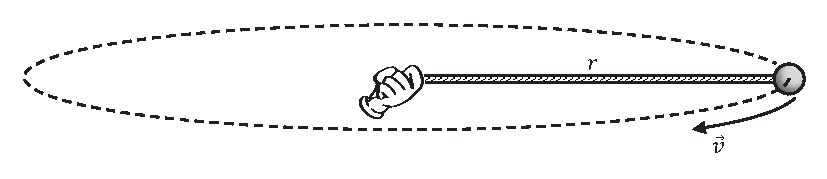
\includegraphics{centripetal/centripetal_fig2_new.eps} \par}
\vspace{0.3cm}

Let's begin our study with some very simple considerations. Suppose an astronaut
goes into outer space, ties a ball to the end of a rope, and spins the ball
so that it moves at a constant speed.

\textbf{Activity 1: Uniform Circular Motion }

(a) Consider the figure above. What is the speed of a ball that moves in a circle
of radius $r = 2.5$ m if it takes 0.50 s to complete one revolution?
\answerspace{20mm}

(b) The speed of the ball is constant! Would you say that this is accelerated
motion?
\answerspace{20mm}

(c) What is the definition of acceleration? (Remember that acceleration is a
vector!)
\answerspace{20mm}

(d) Are velocity and speed the same thing? Is the velocity of the ball constant?
(Hint: Velocity is a vector quantity!)
\answerspace{20mm}

(e) In light of your answers to (c) and (d), would you like to change your answer
to part (b)? Explain.
\answerspace{20mm}

\textbf{Using Vectors to Diagram How Velocity Changes} 

By now you should have concluded that since the direction of the motion of an
object undergoing uniform circular motion is constantly changing, its velocity
is also changing and thus it is accelerating. We would like you to figure out
how to calculate the direction of the acceleration and its magnitude as a function
of the speed v of an object such as a ball as it revolves and as a function
of the radius of the circle in which it revolves. In order to use vectors to
find the direction of velocity change in circular motion, let's review some
rules for adding velocity vectors.

%\vspace{0.3cm}
{\par\centering 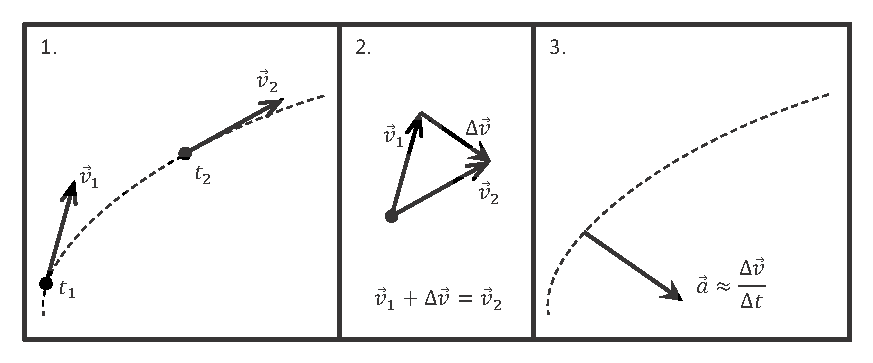
\includegraphics{circ_motion/circ_motion_fig1_new.eps} \par}
%\vspace{0.3cm}

\begin{enumerate}
\item To Draw Velocities: Draw an arrow representing the velocity, \( 
{\vec v}_{1} \), of
the object at time \( t_{1} \). Draw another arrow representing the velocity,
\( {\vec v}_{2} \), of the object at time \( t_{2} \). 
\item To Draw Velocity Change: Find the change in the velocity 
\( \Delta  {\vec v}
= {\vec v}_{2}  - {\vec v}_{1} \) during the time interval described
by \( \Delta  t = t_{2}  - t_{1} \). Start by using the rules of
vector sums to rearrange the terms so that \({\vec v}_{1}  +  \Delta  
{\vec v}
= {\vec v}_{2} \). Next place the tails of the two velocity vectors together
halfway between the original and final location of the object. The change in
velocity is the vector that points from the head of the first velocity vector
to the head of the second velocity vector. 
\item To Draw Acceleration: The acceleration equals the velocity change 
\( \Delta  {\vec v}\)
divided by the time interval $t$ needed for the change. Thus, $\vec a$ is in
the same direction as \( \Delta  {\vec v}\) but is a different length (unless
\( \Delta  t = 1\)). Thus, even if you do not know the time interval, you
can still determine the direction of the acceleration because it points in the
same direction as \( \Delta  {\vec v}\). 
\end{enumerate}
The acceleration associated with uniform circular motion is known as centripetal
acceleration. You will use the vector diagram technique described above to find
its direction. 

\textbf{Activity 2: The Direction of Centripetal Acceleration }

(a) Determine the direction of motion of the ball shown below if it is moving
counter-clockwise at a constant speed. Note that the direction of the ball's
velocity is always tangential to the circle as it moves around. Draw an arrow
representing the direction and magnitude of the ball's velocity as it passes
the dot just before it reaches point A. Label this vector \(\vec v _{1} \). 

%\vspace{0.3cm}
{\par\centering \includegraphics{circ_motion/circ_motion_fig2_new.eps} \par}
%\vspace{0.3cm}

(b) Next, use the same diagram to draw the arrow representing the velocity of
the ball when it is at the dot just after it passes point A. Label this vector
\(\vec{v} _{2} \).

(c) Find the direction and magnitude of the change in velocity as follows. In
the space below, make an exact copy of both vectors, placing the tails of the
two vectors together. Next, draw the vector that must be added to vector \(\vec{v}_{1} \)
to add up to vector \(\vec{v}_{2} \) ; label this vector \( \Delta  \vec {v}\).
Be sure that vectors \(\vec{v}_{1} \) and \(\vec{v}_{2} \) have the
same magnitude and direction in this drawing that they had in your drawing in
part (a)!
\vspace{30mm}

(d) Now, draw an exact copy of \( \Delta  \vec {v}\) on your sketch in part
(a). Place the tail of this copy at point A. Again, make sure that your copy
has the exact magnitude and direction as the original \( \Delta  \vec {v}\)
in part (c).
\vspace{30mm}

(e) Now that you know the direction of the change in velocity, what is the direction
of the centripetal acceleration, \(\vec{a} _{c} \)?
\vspace{20mm}

(f) If you re did the analysis for point B at the opposite end of the circle,
what do you think the direction of the centripetal acceleration, \(\vec{a} _{c} \)),
would be now?
\vspace{20mm}

(g) As the ball moves on around the circle, what is the direction of its acceleration?
\vspace{20mm}

(h) Use Newton's second law in vector form (\( \sum {\vec F} = m{\vec a}\)
) to describe the direction of the net force on the ball as it moves around
the circle.
\vspace{20mm}

(i) If the ball is being twirled around on a string, what is the source of the
net force needed to keep it moving in a circle?
\answerspace{20mm}

\pagebreak[20]
\textbf{Using Mathematics to Derive How Centripetal Acceleration Depends on
Radius and Speed }

You haven't done any experiments yet to see how centripetal acceleration depends
on the radius of the circle and the speed of the object. You can use the rules
of mathematics and the definition of acceleration to derive the relationship
between speed, radius, and magnitude of centripetal acceleration. 

\textbf{Activity 3: How Does \(\vec a _{\rm c} \) Depend on $\vec v$ and $\vec r$?} 

(a) Do you expect you would need more centripetal acceleration or less centripetal
acceleration to cause an object moving at a certain speed to rotate in a smaller
circle? In other words, would the magnitude, \( a_{\rm c} \), have to increase
or decrease as r decreases if circular motion is to be maintained? Explain.
\vspace{20mm}

(b) Do you expect you would need more centripetal acceleration or less centripetal
acceleration to cause an object to rotate at a given radius $r$ if the speed $v$
is increased? In other words, would the magnitude, \( a_{\rm c} \), have to increase
or decrease as $v$ increases if circular motion is to be maintained? Explain.
\vspace{20mm}

You should have guessed that it requires more acceleration to move an object
of a certain speed in a circle of smaller radius and that it also takes more
acceleration to move an object that has a higher speed in a circle of a given
radius. Lets use the definition of acceleration in two dimensions and some accepted
mathematical relationships to show that the magnitude of centripetal acceleration
should actually be given by the equation
\[
a_{\rm c}=\frac{v^{2}}{r}\qquad [Eq.\: 1]\]


In order to do this derivation you will want to use the following definition
for acceleration
\[
\vec a_{\rm avg} =\frac{{{\vec v}_{2}}-{{\vec v}_{1}}}{t_{2}-t_{1}}=\frac{\Delta {\vec v}}{\Delta t}\qquad [Eq.\: 2]\]


\textbf{Activity 4: Finding the Equation for \(a _{\rm c} \) }

(a) Refer to the diagram below. Explain why, at the two points shown on the
circle, the angle between the position vectors at times \( t_{1} \) and \( t_{2} \)
is the same as the angle between the velocity vectors at times \( t_{1} \)
and \( t_{2} \). Hint: In circular motion, velocity vectors are always perpendicular
to their position vectors.

\vspace{0.3cm}
{\par\raggedright \includegraphics{circ_motion/circ_motion_fig3_new.eps} \par}
\vspace{0.3cm}

(b) Since the angles are the same and since the magnitudes of the displacements
never change (i.e., \(r= r_{1}  = r_{2} \)) and the magnitudes of the
velocities never change (i.e., \(v = v_{1}  = v_{2} \)), use the properties
of similar triangles to explain why \( \frac{\Delta v}{v}=\frac{\Delta r}{r} \).
\vspace{20mm}

(c) Now use the equation in part (b) and the definition of 
$ a_{\rm avg} $ to show that
\( (a_{\rm c})_{\rm avg} =\frac{\Delta v}{\Delta t}=\frac{\left( \Delta r\right) }{\left( \Delta t\right) }\frac{v}{r}. \)
\vspace{20mm}

(d) The speed of the object as it rotates around the circle is given by \( v=\frac{\Delta s}{\Delta t} \).
Is the change in arc length, \( \Delta s \), larger or smaller than the magnitude
of the change in the position vector, \( \Delta r \)? Explain why the arc length
change and the change in the position vector are approximately the same when
$t$ is very small (so that the angle $\theta$ becomes very small) i.e., why is
\( \Delta  s
 \simeq   \Delta  r\)?
\vspace{20mm}

(e) If \( \Delta s  \simeq   \Delta  r\), then what is the equation
for the speed in terms of \( \Delta  r\) and \( \Delta  t\)?
\vspace{20mm}

(f) Using the equation in part (c), show that as \( \Delta t  \rightarrow 0 \),
the instantaneous value of the centripetal acceleration is given by Eq. 1.
\vspace{20mm}

(g) If the object has a mass $m$, what is the equation for the magnitude of the
centripetal force needed to keep the object rotating in a circle (in terms of
$v$, $r$, and $m$)? In what direction does this force point as the object rotates
in its circular orbit?
\vspace{20mm}

\textbf{Experimental Test of the Centripetal Force Equation }

The theoretical considerations in the last activity should have led you to the
conclusion that, whenever you see an object of mass m moving in a circle of
radius $r$ at a constant speed $v$, it must at all times be experiencing a net centripetal
force directed toward the center of the circle that has a magnitude of
\[
F_{\rm c}=ma_{\rm c}=m\frac{v^{2}}{r}\qquad [Eq.\: 3]\]


Let's check this out. Does this rather odd equation really work for an external
force?

To test the validity of the derivation we must compare it to experience. We
will use a ``toy'' airplane suspended from a string and flying
in a circular path. We will use the video analysis system to measure the properties
of the motion and determine the horizontal and vertical components of the force
exerted on the airplane using Equation 3. We will compare that result with a
direct measurement of the tension in the string. 

\textbf{Activity 5: Verifying the \(F_{\rm c} \) Equation }

(a) Measure the mass of the airplane and the length $L$ of the portion of the
string that hangs below the horizontal post with the hole in it. Record the
values here: 
\vspace{10mm}

(b) The airplane is suspended from a spring scale. The string should pass straight
down from the scale through the small hole in the horizontal post. The camera
should be placed 1 to 2 meters above the airplane looking down. Turn on the camera and center
the spring scale in the frame. In order to turn on the camera, you will have to open ``\textbf{Camera}'' (see \textbf{Appendix \ref{tracker}: Video Analysis Using Tracker}). Check that the reading of the spring
scale is consistent with the mass of the airplane. Mount a ruler somewhere in the
camera's field of view to serve as a scaling object. Launch the plane into uniform
circular motion. When the motion is steady record a movie of at least one complete
revolution and record the reading of the spring scale here:
\vspace{5mm}

\hspace{0.5in} \( F_{\rm scale} \) = 
\vspace{5mm}

%(c) Determine the position of the airplane during one complete revolution. If using \textbf{VideoPoint}, follow the instructions in the second section of 
%\textbf{Appendix D: Video Analysis} for recording and calibrating a data file.
%As you analyze the movie frame by frame, estimate to the nearest fraction
%of a frame the number of frames for one complete revolution. Record your result below.
%When you calibrate the time and position data, note the number of frames per
%second of the movie and convert that number to the time interval between frames,
%\( \Delta  t\). Record this result below. Now you can determine the time interval for 
%one complete revolution and record it below. The resulting data file should contain three columns with the values of
%time, x-position, and y-position.
%
%\hspace{0.5in} \( N_{frame} \) = 
%
%\hspace{0.5in} \( \Delta t \) = 
(c) To analyze the movie, use \textit{Tracker} (see \textbf{Appendix \ref{tracker}: Video Analysis Using Tracker}). 
Set the origin of coordinate axes at the axis of revolution of the plane.  After your track is made for one complete revolution, make a graph of $x$ vs $t$. Double click on the graph to expand it, print the graph and include with this unit. Read the period of revolution for the complete cycle and record it here:
\vspace{5mm}

\hspace{0.5in} \( t_{\rm rev} \) = 
\vspace{5mm}

%(d) Make a graph of the trajectory of the airplane during one full revolution.
%See \textbf{Appendix \ref{excel}: Introduction to Excel} for details on using
%the graphing software. When you make your plot make sure the x and y axes cover
%the same size range; otherwise, 
%you will distort the path of the airplane. Print
%your plot and attach it to your write-up.

%\begin{enumerate}
%\item Is the motion circular? What is your evidence?\vspace{10mm}
%
%\item What is the radius of the motion? $r =$
%\end{enumerate}
(d) Next, make a graph of $y$ vs $x$.  Result will be a circle. Double click on the graph to expand it, read the diameter of the circle from the graph, and record the radius of the path here:
\vspace{5mm}

\hspace{0.5in} $r =$
\vspace{5mm}

Print the graph and include with this unit.

(e) To test the validity of the expression for \( F_{\rm c} \) we must know the
speed. Use the measurements of the radius of the airplane's trajectory and the
time for one complete revolution to calculate the average speed.
\vspace{5mm}

\hspace{0.5in} \( v_{\rm ave} \) = 
\vspace{5mm}

(f) Use your results for the mass, the average velocity of the airplane, and
the radius of the circular motion to predict the centripetal force exerted by
the string.
\vspace{5mm}

\hspace{0.5in} \( F_{\rm c} \) = 
\vspace{5mm}

(g) We will now determine the net force exerted by the string on the airplane
by using a little trigonometry.
Recall that we know $r$, the radius of the airplane's circular path, and 
$L$, the total length of the string that is actually rotating. 

\begin{enumerate}
\item Using these two distances ($r$ and $L$), 
calculate the angle the string makes with
the horizontal. You may want to draw a diagram to do this. 

\bigskip
\( \theta  =\)  \vspace{5mm}

\item We determined the horizontal component of the force on the airplane 
\( F_{\rm c} \) in part (f). Knowing the angle \( \theta \) we can determine an
expression for the
net force exerted by the string on the airplane, \( F_{\rm plane} \). Draw a vector
force diagram including \( F_{\rm c} \) and \( F_{\rm plane} \), derive an expression
for \( F_{\rm plane} \), calculate it, and record it here: 

\bigskip
\( F_{\rm plane} =\)  \vspace{10mm}

\end{enumerate}
(h) Compare your result for \( F_{\rm plane} \) with the measurement of the spring
scale \( F_{\rm scale} \). Should they be different? Should they be the same? Explain.
\vspace{15mm}


(i) Calculate the difference between \( F_{\rm plane} \) and \( F_{\rm scale} \) (\( F_{\rm plane} - F_{\rm scale} \))and record it below.
Go around to the other lab groups and get their results for this quantity.
Make a histogram of the results you collect and calculate the average and standard deviation.
For information on making histograms, see \textbf{Appendix \ref{excel}}. For information on calculating the average and
standard deviation, see \textbf{Appendix \ref{treatment}}. Record the average and standard deviation here.
Attach the histogram to this unit.
\vspace{30mm}

(j) What is your expectation for the difference \( F_{\rm plane} - F_{\rm scale} \)?
Do the data from the class support this expectation? 
Use the average and standard deviation for the class to quantitatively answer this question.
\vspace{20mm}

(k) What does the histogram of the class data tell you?
\vspace{20mm}

(l) Discuss the major sources of uncertainty in this experiment.
\vspace{15mm}

